
\section{Spatial Controls at Matched Realized Correction RMS}
\label{sec:r86-details}
\subsection{Population, intervention, and evaluation}
This follow-up addresses the realized-dose drift of the main CORR25--ENERGY comparison. Ten previously evaluated benchmark sources are selected by ascending SHA256 of the ASCII string \texttt{R86-pilot-20261103:<case ID>}; each uses seed 0. These are seen sources, not an additional independent test population. The two designated direction contrasts are request versus global and request versus shifted support at the original magnitude profile. All ten selected cases are retained.

For source $s$ and step $i$, let $b_{s,i}=\operatorname{RMS}(\widehat c^{\rm anchor}_{s,i})$ be the recorded CORR25 correction magnitude. Each branch evaluates its direction $v_i$ at its own current state and applies Eq.~\eqref{eq:r86-profile}.
The directions are $P\odot c_i$ (request), the nonzero full-image residual $c_i$ (global), and $\widetilde P\odot c_i$ (shift). The shift control rolls $P$ by 32 cells along both axes of the $64\times64$ grid with wraparound, preserving all map values and support area. The time grid, prompts, source memory, and initial state remain fixed. There is no gain cap. The nonzero norms in the completed runs allow Eq.~\eqref{eq:r86-profile} to realize the assigned profile at every step. Matching actual norms controls the magnitudes and their timing; spatial direction, net vector displacement, and the target field's state-dependent response remain free to differ.

The original request/$1.0$ outputs are reused as anchors. Shift/$1.0$, global/$1.0$, request/$0.7$, and global/$0.7$ each produce ten new outputs: 40 new generations and 50 evaluated arm--source records including the anchors. All 40 new generations and automatic evaluations complete successfully. The ten anchors also have complete automatic scores. Full-image and text metrics use ten sources; preservation metrics use nine because the cloud-scene request has an empty preservation complement. Scores are computed from native PNGs on the server with the same CLIP, DINOv2, and LPIPS weights as the benchmark. The compact result archive retains these scores and previews rather than native output PNGs. No new VLM ratings are collected.

Across $40\times28=1,120$ new steps, the maximum absolute applied-RMS discrepancy is $5.96\times10^{-8}$ and the maximum relative discrepancy from $\beta b_{s,i}$ is $1.52\times10^{-7}$. Each generated branch costs 97 NFE, totaling 3,880 new calls. Obtaining a new anchor and one branch from scratch costs $97+97=194$ calls; this study reuses the available anchors. The profile-control arms are attribution experiments rather than standalone low-cost editors.

\subsection{All operating points and paired inference}
Table~\ref{tab:r86-means} gives all five operating points. On the nine regional sources, Request/Global/Shift preservation LPIPS is 0.5920/0.6042/0.6134 at scale 1.0; request-minus-comparator differences are $-0.0122/-0.0215$, with $p_{H12}=0.344/0.156$. At fixed magnitudes, request routing has lower mean LPIPS and preservation MAE than global and shifted directions. At either request or global allocation, reducing the assigned profile to $0.7$ raises LPIPS and preservation MAE. Text and DINO responses are smaller and variable.

\begin{table*}[t]
\centering\small
\caption{All realized-magnitude controls. Each row contains ten seed-0 outputs; preservation LPIPS and MAE use nine nonempty complements. The request/$1.0$ row reuses benchmark anchors. Means are descriptive, with paired inference in Table~\ref{tab:r86-primary}.}
\label{tab:r86-means}
\setlength{\tabcolsep}{4pt}
\begin{tabular}{lrrrrrr}
\toprule
Direction / scale & Target CLIP $\uparrow$ & Dir. CLIP $\uparrow$ & DINO $\uparrow$ & LPIPS full $\downarrow$ & LPIPS pres. $\downarrow$ & Pres. MAE $\downarrow$\\
\midrule
Request / 1.0 (reused) & 0.2439 & 0.1582 & 0.5487 & 0.5900 & 0.5920 & 0.1436\\
Global / 1.0 & 0.2473 & 0.1567 & 0.5508 & 0.5975 & 0.6042 & 0.1508\\
Shift / 1.0 & 0.2469 & 0.1589 & 0.5503 & 0.6048 & 0.6134 & 0.1603\\
Request / 0.7 & 0.2456 & 0.1605 & 0.5474 & 0.6415 & 0.6455 & 0.1850\\
Global / 0.7 & 0.2503 & 0.1605 & 0.5406 & 0.6447 & 0.6531 & 0.1890\\
\bottomrule\end{tabular}\end{table*}

Pointwise percentile intervals use 10,000 source-bootstrap resamples with seed 86001. The two-sided sign-flip test enumerates all $2^n$ source-sign assignments. Table~\ref{tab:r86-primary} reports raw $p$, Holm correction across the two direction contrasts separately for each endpoint ($p_{H2}$), and correction across both contrasts and all six endpoints ($p_{H12}$). The protocol designates the two direction contrasts but no unique primary endpoint or fully specified multiplicity family; both correction scopes are reported as analysis choices. Pointwise intervals and adjusted tests answer different uncertainty questions.

\begin{table*}[t]
\centering\small
\caption{Request minus comparator at profile scale 1.0. Negative LPIPS/MAE differences favor request routing. Sources are the independent sampling units within this follow-up; all are previously evaluated benchmark cases. Intervals are pointwise, while $p_{H2}$ and $p_{H12}$ adjust the stated families.}
\label{tab:r86-primary}
\setlength{\tabcolsep}{5pt}
\begin{tabular}{llrrrrrr}
\toprule
Comparator & Metric & Sources & Difference & 95\% CI & $p$ & $p_{H2}$ & $p_{H12}$\\
\midrule
Global & Target CLIP & 10 & $-0.0033$ & $[-0.0128,+0.0046]$ & 0.5703 & 1.0000 & 1.0000\\
Global & Directional CLIP & 10 & $+0.0015$ & $[-0.0101,+0.0140]$ & 0.8281 & 1.0000 & 1.0000\\
Global & DINO & 10 & $-0.0021$ & $[-0.0293,+0.0325]$ & 0.9160 & 1.0000 & 1.0000\\
Global & LPIPS full & 10 & $-0.0075$ & $[-0.0153,-0.0003]$ & 0.1016 & 0.1016 & 0.7109\\
Global & LPIPS pres. & 9 & $-0.0122$ & $[-0.0210,-0.0025]$ & 0.0430 & 0.0430 & 0.3438\\
Global & Pres. MAE & 9 & $-0.0072$ & $[-0.0109,-0.0035]$ & 0.0078 & 0.0156 & 0.0938\\
Shift & Target CLIP & 10 & $-0.0030$ & $[-0.0117,+0.0041]$ & 0.5527 & 1.0000 & 1.0000\\
Shift & Directional CLIP & 10 & $-0.0008$ & $[-0.0134,+0.0119]$ & 0.9160 & 1.0000 & 1.0000\\
Shift & DINO & 10 & $-0.0016$ & $[-0.0307,+0.0304]$ & 0.9316 & 1.0000 & 1.0000\\
Shift & LPIPS full & 10 & $-0.0148$ & $[-0.0240,-0.0054]$ & 0.0156 & 0.0312 & 0.1562\\
Shift & LPIPS pres. & 9 & $-0.0215$ & $[-0.0330,-0.0101]$ & 0.0156 & 0.0312 & 0.1562\\
Shift & Pres. MAE & 9 & $-0.0167$ & $[-0.0272,-0.0072]$ & 0.0078 & 0.0156 & 0.0938\\
\bottomrule\end{tabular}\end{table*}

Request minus global preservation LPIPS is $-0.0122$ ($[-0.0210,-0.0025]$); request minus shift is $-0.0215$ ($[-0.0330,-0.0101]$). Their $p_{H2}$ values are 0.0430 and 0.0313, while $p_{H12}$ values are 0.3438 and 0.1563. The full-image request--global bootstrap interval excludes zero, but its exact sign-flip $p=0.1016$; this difference reflects the small sample and distinct inference procedures. The two designated directional-CLIP intervals span zero, leaving semantic differences unresolved rather than establishing equivalence. The fixed-profile results add a direction-sensitive retention observation after numerical dose drift is removed; broad-family inference remains limited at this sample size.

\begin{figure}[t]
\centering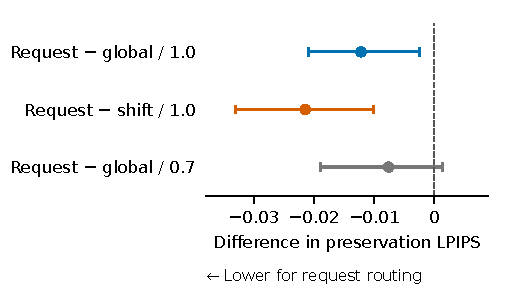
\includegraphics[width=\columnwidth]{figures/r86_actual_dose.pdf}
\caption{Realized-profile direction contrasts. All intervals resample sources; nine sources enter preservation LPIPS. The 0.7 contrast is exploratory.}
\label{fig:r86-supp-effects}
\end{figure}

\subsection{Reduced magnitude and interaction}
On the same nine regional sources, the post-hoc preservation-LPIPS difference for $\beta=0.7$ minus $1$ is $+0.0535$ (pointwise 95\% CI $[0.0302,0.0808]$) for request and $+0.0489$ ($[0.0259,0.0784]$) for global correction. The direction-by-dose interaction remains $-0.0046$ ($[-0.0172,0.0079]$).

Table~\ref{tab:r86-secondary} retains the exploratory reduced-profile contrast and the difference between direction contrasts at the two scales. Request minus global preservation LPIPS is $-0.0076$ at scale 0.7, with interval $[-0.0189,0.0015]$. The difference of the two LPIPS contrasts is $-0.0046$ ($[-0.0172,0.0079]$). Thus the observed allocation advantage is smaller at the reduced profile, but the interaction's uncertainty does not establish a dose-dependent LPIPS allocation effect.

\begin{table*}[t]
\centering\small
\caption{Exploratory reduced-profile effects and interaction: $(\mathrm{Request}-\mathrm{Global})_{1.0}-(\mathrm{Request}-\mathrm{Global})_{0.7}$. Pointwise source-bootstrap intervals; these secondary contrasts are outside the 12-test family above.}
\label{tab:r86-secondary}
\begin{tabular}{lrrrrr}
\toprule
Metric & Sources & Difference at 0.7 & 95\% CI & Interaction & 95\% CI\\
\midrule
Target CLIP & 10 & $-0.0047$ & $[-0.0139,+0.0057]$ & $+0.0013$ & $[-0.0076,+0.0100]$\\
Directional CLIP & 10 & $+0.0001$ & $[-0.0047,+0.0053]$ & $+0.0014$ & $[-0.0117,+0.0158]$\\
DINO & 10 & $+0.0068$ & $[-0.0180,+0.0292]$ & $-0.0088$ & $[-0.0341,+0.0188]$\\
LPIPS full & 10 & $-0.0033$ & $[-0.0088,+0.0020]$ & $-0.0043$ & $[-0.0138,+0.0044]$\\
LPIPS pres. & 9 & $-0.0076$ & $[-0.0189,+0.0015]$ & $-0.0046$ & $[-0.0172,+0.0079]$\\
Pres. MAE & 9 & $-0.0040$ & $[-0.0080,-0.0003]$ & $-0.0033$ & $[-0.0051,-0.0016]$\\
\bottomrule\end{tabular}\end{table*}

\paragraph{Post-hoc fixed-direction dose contrasts.}
Table~\ref{tab:r86-dose-paired} compares $\beta=0.7$ minus $1$ within each direction on the same nine sources with nonempty preservation regions. The request means are 0.6454929 and 0.5919901; global means are 0.6530523 and 0.6041709. These newly added post-hoc contrasts use existing outcomes. Each pointwise 95\% interval uses 10,000 paired source-bootstrap draws, seeds 86201 (request) and 86202 (global), and zero-based sorted positions 250 and 9749. Two-sided exact sign flips enumerate all $2^9$ assignments. Holm adjustment is applied only to these two post-hoc dose tests, separately from the earlier 12-test direction family. The new contrasts are recorded in \texttt{evidence/review\_additions/}; the direction-by-dose interaction above is unchanged.

\begin{table*}[t]
\centering\small
\caption{Post-hoc preservation-LPIPS dose contrasts, $\beta=0.7$ minus $1$, at fixed direction. Each row uses nine paired sources. CIs are pointwise; $p_{H2,\mathrm{dose}}$ adjusts only these two dose tests.}
\label{tab:r86-dose-paired}
\begin{tabular}{lrrrr}
\toprule
Direction & Difference & 95\% CI & Exact $p$ & $p_{H2,\mathrm{dose}}$\\
\midrule
Request & $+0.0535$ & $[0.0302,0.0808]$ & 0.0039 & 0.0078\\
Global & $+0.0489$ & $[0.0259,0.0784]$ & 0.0039 & 0.0078\\
\bottomrule
\end{tabular}
\end{table*}

\subsection{Response localization and visible outcomes}
The localization diagnostic is $L=\operatorname{mean}_{\rm edit}(E)-\operatorname{mean}_{\rm preserve}(E)$, using official masks only for evaluation. On nine eligible sources, its exported mean is 0.3002 for the native request response and $-0.0618$ for its shifted version. The native value is larger on eight of nine sources; the couch case reverses this direction. Native floating-point response arrays are recorded for the new branches. The original anchor archive contains only map previews, so this diagnostic uses the regenerated fixed-reference response from the request/$0.7$ branch, not a claimed recovery of the original anchor tensor. Official region masks are BOX-resampled to the $64\times64$ response grid. The compact package includes localization values and metadata; those values cannot be independently regenerated from the compact package alone because the official mask images are not included.

Figures~\ref{fig:r86-gallery1} and~\ref{fig:r86-gallery2} show every selected task and all five arms. Tulip recoloring and camera-to-phone replacement visibly occur, accompanied by changed composition or person details. In the wing-removal task, wings remain in every arm; the haircut request changes the front-facing portrait into a rear view. These observations retain the distinction between measured source retention and completion of the full request. The pilot isolates correction direction at fixed amplitudes, conditional on the frozen profile and editor; Section~\ref{sec:r87-fresh} tests the direction effect on fresh sources.

\begin{figure*}[t]
\centering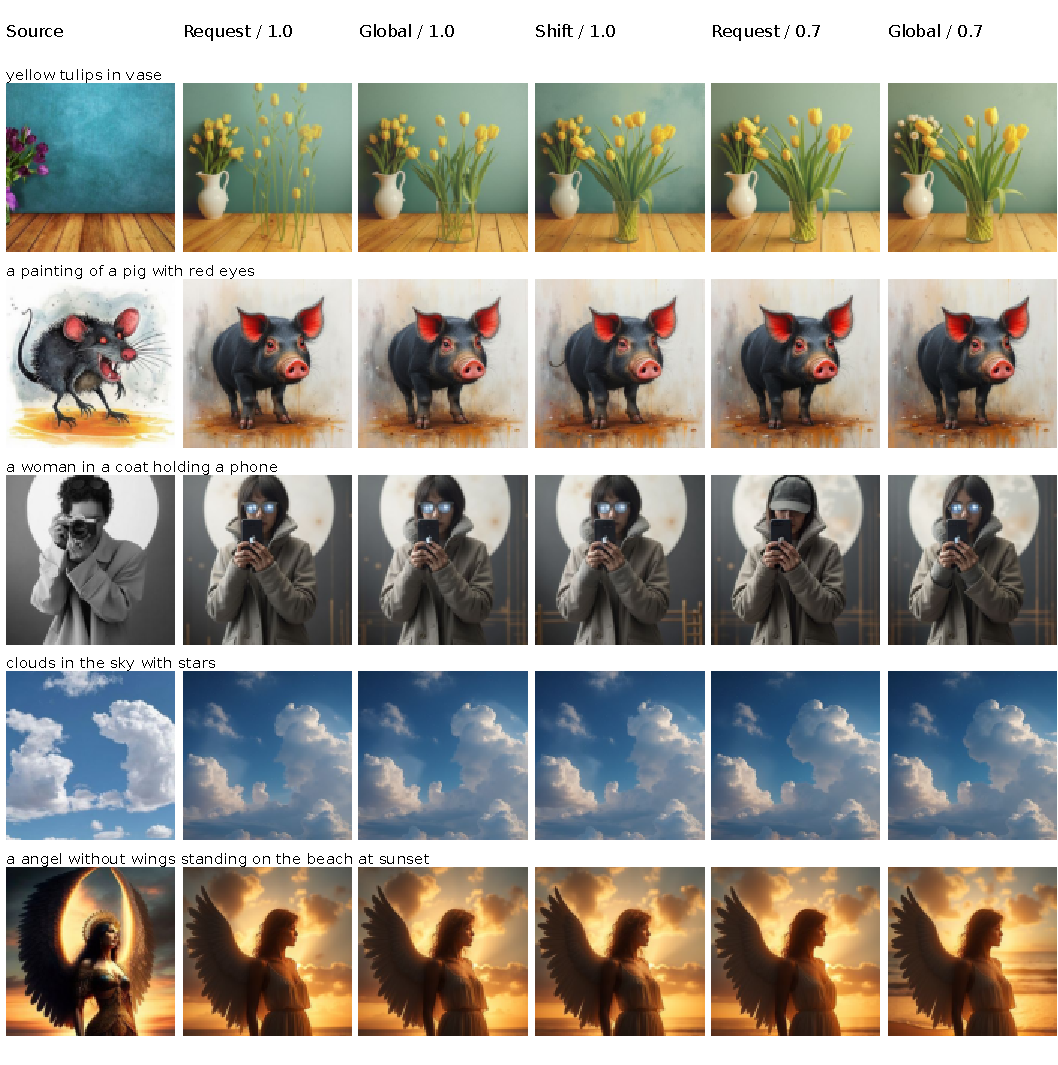
\includegraphics[width=\textwidth]{figures/r86_gallery_1.pdf}
\caption{All five realized-profile controls for the first five selected cases. Each row shows the target prompt and unchanged full-frame previews. The request/$1.0$ column reuses the original CORR25 anchor.}
\label{fig:r86-gallery1}
\end{figure*}
\begin{figure*}[t]
\centering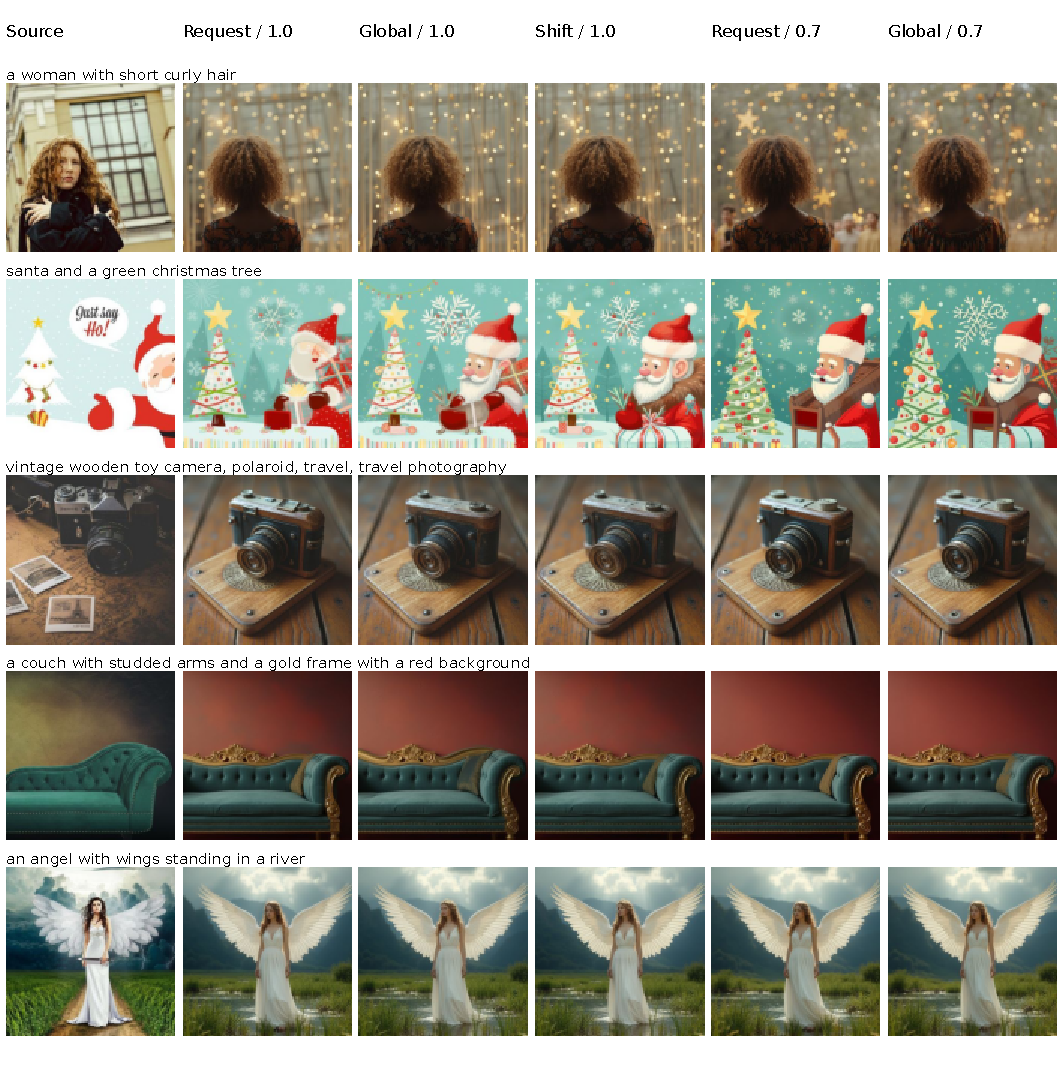
\includegraphics[width=\textwidth]{figures/r86_gallery_2.pdf}
\caption{Remaining five selected cases, with the same column order and full-frame previews. The haircut row illustrates a major viewpoint change shared across all arms; the camera and angel rows also retain substantial source departures.}
\label{fig:r86-gallery2}
\end{figure*}

\subsection{Fresh-source confirmation}
Section~\ref{sec:r87-fresh} reports the completed extension: twenty fresh sources, two seeds, and request, global, shifted, and block-permuted directions at matched realized stepwise RMS. All 160 outputs and their automatic metrics are complete. The pilot supplies the fixed-direction dose contrasts; the fresh-source study tests the spatial findings on a separately selected population.
